\documentclass[12pt,a4paper]{article}

%====================================================
% PACKAGES
%====================================================

\usepackage[utf8]{inputenc}
\usepackage[T1]{fontenc}
\usepackage[a4paper,margin=0.85in]{geometry}
\usepackage[siunitx]{circuitikz}
\usepackage{sansmath}
\usepackage{amssymb}
\usepackage{graphicx}
\usepackage{enumitem}
\usepackage{booktabs}
\usepackage{array}
\usepackage{hyperref}
\usepackage{circuitikz}
\usepackage{amsmath} % Added to support math text commands safely
\usepackage[many]{tcolorbox}
\tcbuselibrary{skins,breakable}

\usepackage{tikz}
\usetikzlibrary{
arrows.meta,
positioning,
calc,
shapes.geometric,
backgrounds
}
\usetikzlibrary{circuits.logic.US, positioning, calc}

\usepackage{fancyhdr}
\usepackage{xcolor}
\definecolor{accent}{RGB}{0,120,215}
\usepackage[scaled=0.90]{helvet}
\renewcommand{\familydefault}{\sfdefault}
\hypersetup{
    colorlinks=true,
    linkcolor=black,
    urlcolor=blue,
    citecolor=black
}
%====================================================
% MONOCHROME THEME
%====================================================

\definecolor{primary}{HTML}{111111}
\definecolor{secondary}{HTML}{2D2D2D}
\definecolor{lightgray}{HTML}{EAEAEA}
\definecolor{bg}{HTML}{F8F8F8}
\definecolor{textgray}{HTML}{555555}

%====================================================
% PAGE STYLE
%====================================================

\pagestyle{fancy}

\fancyhf{}

\fancyfoot[L]{Digital Logic Hardware Implementation}
\fancyfoot[R]{\thepage}

\renewcommand{\familydefault}{\sfdefault}
\renewcommand{\headrulewidth}{0pt}
\renewcommand{\footrulewidth}{0.4pt}

%====================================================
% QUESTION BOX
%====================================================

\newtcolorbox{questionbox}{
enhanced,
breakable,
colback=bg,
colframe=primary,
boxrule=0pt,
leftrule=5pt,
sharp corners,
title=\textbf{PROBLEM STATEMENT},
fonttitle=\large\bfseries,
coltitle=primary,
boxed title style={
    colback=black,
    colframe=black
},
coltitle=white,
top=12pt,bottom=12pt,left=14pt,right=14pt
}

%====================================================
% TRUTH TABLE BOX
%====================================================

\newtcolorbox{truthtablebox}{
    enhanced,
    breakable,
    colback=gray!2,
    colframe=black,
    boxrule=0.8pt,
    sharp corners,
    title=\textbf{TRUTH TABLE ANALYSIS},
    fonttitle=\large\bfseries,
    coltitle=black,
boxed title style={
    colback=black,
    colframe=black
},
coltitle=white,
    top=12pt,
    bottom=12pt,
    left=14pt,
    right=14pt
}

%====================================================
% SOLUTION BOX
%====================================================

\newtcolorbox{solutionbox}{
enhanced,
breakable,
colback=white,
colframe=primary,
boxrule=0pt,
leftrule=5pt,
sharp corners,
title=\textbf{STEP-BY-STEP DERIVATION},
fonttitle=\large\bfseries,
coltitle=primary,
boxed title style={
    colback=black,
    colframe=black
},
coltitle=white,
top=12pt,bottom=12pt,left=14pt,right=14pt
}

%====================================================
% HARDWARE BOX
%====================================================

\newtcolorbox{hardwarebox}{
enhanced,
breakable,
colback=white,
colframe=primary,
boxrule=0pt,
leftrule=5pt,
sharp corners,
title=\textbf{HARDWARE IMPLEMENTATION},
fonttitle=\large\bfseries,
coltitle=primary,
boxed title style={
    colback=black,
    colframe=black
},
coltitle=white,
top=12pt,bottom=12pt,left=14pt,right=14pt
}

%====================================================
% CIRCUIT BOX
%====================================================

\newtcolorbox{circuitbox}{
enhanced,
breakable,
colback=bg,
colframe=primary,
boxrule=1pt,
sharp corners,
title=\textbf{HARDWARE BLOCK DIAGRAM},
fonttitle=\large\bfseries,
coltitle=primary,
boxed title style={
    colback=black,
    colframe=black
},
coltitle=white,
top=14pt,bottom=14pt,left=14pt,right=14pt
}

%====================================================
% CODE BOX
%====================================================

\newtcolorbox{codebox}{
    enhanced,
    breakable,
    colback=gray!2,
    colframe=black,
    boxrule=0.8pt,
    sharp corners,
    title=\textbf{SOURCE CODE REPOSITORIES},
    fonttitle=\large\bfseries,
    coltitle=black,
boxed title style={
    colback=black,
    colframe=black
},
coltitle=white,
    top=12pt,
    bottom=12pt,
    left=14pt,
    right=14pt
}


%====================================================
% RESULT BOX
%====================================================

\newtcolorbox{resultbox}{
enhanced,
breakable,
colback=success!5,
colframe=success,
boxrule=1pt,
sharp corners,
title=\textbf{FINAL RESULT},
fonttitle=\large\bfseries,
coltitle=success,
boxed title style={
    colback=black,
    colframe=black
},
coltitle=white,
top=12pt,
bottom=12pt,
left=12pt,
right=12pt
}

%====================================================
% HYPERLINK COLORS
%====================================================

\hypersetup{
colorlinks=true,
linkcolor=accent,
urlcolor=accent,
citecolor=accent
}

\newtcolorbox{linkbox}{
    enhanced,
    colback=white,
    colframe=black!60,
    boxrule=0.8pt,
    arc=3pt,
    left=6pt,
    right=6pt,
    top=4pt,
    bottom=4pt,
    width=0.9\linewidth
}

%====================================================
% TABLE SPACING
%====================================================

\renewcommand{\arraystretch}{1.4}

\begin{document}

\begin{titlepage}
\centering

\vspace*{2.5cm}

{\Huge\bfseries Digital Logic Hardware Implementation}

\vspace{0.4cm}

\rule{0.55\textwidth}{0.8pt}

\vspace{0.4cm}

{\Large GATE EC 2014 Circuit Analysis}

\vspace{2cm}

{\Large H B S Bharath Kumar}

\vspace{0.3cm}

{\large M.Sc Artificial Intelligence}

\vfill

\rule{0.35\textwidth}{0.5pt}

\vspace{0.3cm}

{\large \today}

\end{titlepage}

\begin{questionbox}

\vspace{0.5cm}
\textbf{Q37.} Consider the circuit shown in Fig. 3.20. If
$C=0$ the expression for $Y$ is

\vspace{0.3cm}

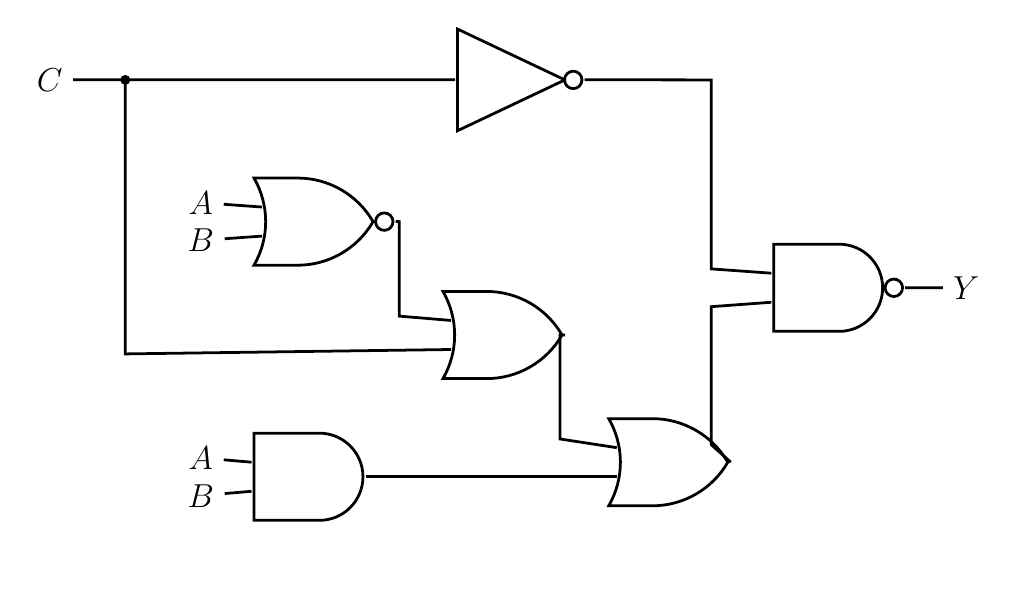
\begin{tikzpicture}[circuit logic US, every circuit symbols/.style={line width=1.2pt}, line width=1pt, scale=1.2]

    % ==================== LOGIC GATES DEFINITION ====================
    % Top path NOT gate
    \node [not gate, scale=1.5] (not1) at (4.5, 5.0) {};
    
    % Upper middle NOR gate
    \node [nor gate, scale=1.5, inputs={nn}] (nor1) at (2.5, 3.5) {};
    
    % Middle stage OR gate
    \node [or gate, scale=1.5, inputs={nn}] (or1) at (4.5, 2.3) {};
    
    % Bottom path AND gate
    \node [and gate, scale=1.5, inputs={nn}] (and1) at (2.5, 0.8) {};
    
    % Bottom stage OR gate - Anchored precisely to AND1's output level for a perfectly straight line
    \node [or gate, scale=1.5, inputs={nn}, anchor=input 2] (or2) at (5.8, 0.8) {};
    
    % Final stage NAND gate
    \node [nand gate, scale=1.5, inputs={nn}] (nand1) at (8.0, 2.8) {};


    % ==================== INPUT LABELS ====================
    % Input C
    \node (C) at (-0.2, 5.0) {\large $C$};
    
    % Inputs for NOR gate (A, B)
    \node (A1) at (1.4, 3.7) {\large $A$};
    \node (B1) at (1.4, 3.3) {\large $B$};
    
    % Inputs for AND gate (A, B)
    \node (A2) at (1.4, 1.0) {\large $A$};
    \node (B2) at (1.4, 0.6) {\large $B$};


    % ==================== CONNECTIONS & ROUTING ====================
    
    % 1. Input C straight to NOT gate
    \draw (C) -- (not1.input);
    
    % 2. Branch from line C down BEFORE the labels to prevent any intersections
    \draw (0.6, 5.0) -- (0.6, 2.1) -- (or1.input 2);
    \fill (0.6, 5.0) circle (1.5pt);
    
    % 3. Connect inputs A and B straight into NOR gate
    \draw (A1) -- (nor1.input 1);
    \draw (B1) -- (nor1.input 2);
    
    % 4. Connect NOR gate output to top input of middle OR gate
    \draw (nor1.output) -- (3.5, 3.5) -- (3.5, 2.5) -- (or1.input 1);
    
    % 5. Connect inputs A and B straight into AND gate
    \draw (A2) -- (and1.input 1);
    \draw (B2) -- (and1.input 2);
    
    % 6. Connect middle OR gate output down to bottom OR gate 
    % Fixes the overlap: drop down at x=5.2, then enter input 1 horizontally
    \draw (or1.output) -| (5.2, 1.2) -- (or2.input 1);
    
    % 7. Connect AND gate output straight into bottom input of bottom OR gate (Guaranteed perfectly straight)
    \draw (and1.output) -- (or2.input 2);
    
    % 8. Route NOT gate output to final NAND gate top input
    \draw (not1.output) -- (6.8, 5.0) -- (6.8, 3.0) -- (nand1.input 1);
    
    % 9. Route bottom OR gate output to final NAND gate bottom input
    \draw (or2.output) -- (6.8, 1.14) -- (6.8, 2.6) -- (nand1.input 2);


    % ==================== OUTPUT LABEL ====================
    \node (Y) at (9.5, 2.8) {\large $Y$};
    \draw (nand1.output) -- (Y);

    % Figure caption
    \node[below=0.6cm of or2, xshift=-1.3cm, font=\sffamily\large] {};

\end{tikzpicture}

\vspace{0.2cm}

\begin{enumerate}[label=\textbf{\alph*)}]
\item $A\bar B+\bar AB$
\item $A+B$
\item $\bar A+\bar B$
\item $AB$
\end{enumerate}

\end{questionbox}
\begin{truthtablebox}

\vspace{0.25cm}
\begin{center}
\renewcommand{\arraystretch}{1.4}
\setlength{\tabcolsep}{12pt}

\begin{tabular}{|c|c||c|c|c||c|}
\hline
\textbf{A} & \textbf{B} &
$\mathbf{X=\overline{A+B}}$ &
$\mathbf{Q=AB}$ &
$\mathbf{R=X+Q}$ &
$\mathbf{Y=\overline{R}}$
\\
\hline

0 & 0 & 1 & 0 & 1 & \textbf{0} \\
\hline

0 & 1 & 0 & 0 & 0 & \textbf{1} \\
\hline

1 & 0 & 0 & 0 & 0 & \textbf{1} \\
\hline

1 & 1 & 0 & 1 & 1 & \textbf{0} \\
\hline

\end{tabular}
\end{center}
\end{truthtablebox}
\newpage

\begin{solutionbox}

\textbf{Step 1: Evaluate the Upper NOR Gate} \\

The upper-left gate is a NOR gate with inputs $A$ and $B$.

\[
X=\overline{A+B}
\]

Applying De Morgan's theorem,

\[
X=\bar A\bar B
\]

Thus, the output of the NOR gate is

\[
\boxed{X=\bar A\bar B}
\]

\vspace{0.3cm}

\textbf{Step 2: Evaluate the First OR Gate} \\

The output of the NOR gate is ORed with the input $C$.

\[
P=X+C
\]

Substituting $X=\bar A\bar B$,

\[
P=\bar A\bar B+C
\]

Since the problem specifies

\[
C=0
\]

therefore

\[
P=\bar A\bar B
\]

\vspace{0.3cm}

\textbf{Step 3: Evaluate the Lower AND Gate} \\

The lower gate is an AND gate with inputs $A$ and $B$.

\[
Q=AB
\]

Thus, the output of the AND gate is

\[
\boxed{Q=AB}
\]

\vspace{0.3cm}

\textbf{Step 4: Evaluate the Second OR Gate} \\

The outputs $P$ and $Q$ are applied to the next OR gate.

\[
R=P+Q
\]

Substituting the obtained expressions,

\[
R=\bar A\bar B+AB
\]

\vspace{0.3cm}
\textbf{Step 5: Evaluate the Inverter Branch} \\

Input $C$ is also connected to a NOT gate.

Since

\[
C=0
\]

the inverter output becomes

\[
\bar C = 1
\]

\vspace{0.3cm}

\textbf{Step 6: Evaluate the Final NAND Gate} \\

The final gate is a NAND gate whose inputs are $R$ and $\bar C$.

\[
Y=\overline{R\cdot\bar C}
\]

Substituting $\bar C=1$,

\[
Y=\overline{R\cdot1}
\]

\[
Y=\overline{R}
\]

Substituting the value of $R$,

\[
Y=\overline{\bar A\bar B+AB}
\]

Applying De Morgan's theorem,

\[
Y=(\bar A\bar B)'(AB)'
\]

\[
Y=(A+B)(\bar A+\bar B)
\]

Expanding,

\[
Y=A\bar B+\bar AB
\]

\vspace{0.3cm}

Hence, the given circuit realizes the Exclusive-OR (XOR) function.

\[
\boxed{Y=A\bar B+\bar AB}
\]

\begin{center}

\begin{tcolorbox}[
width=0.55\textwidth,
colback=white,
colframe=black,
boxrule=0.8pt,
sharp corners,
center title,
halign=center
]

\textbf{\Large Correct Option : (a)}

\vspace{0.15cm}

\[
\boxed{A\bar B+\bar AB}
\]

\end{tcolorbox}

\end{center}

\end{solutionbox}

\begin{hardwarebox}

\textbf{1. Components Required}

\begin{itemize}[itemsep=0.1em]
\item 1x Arduino UNO
\item 1x Breadboard
\item 2x Push Buttons (Inputs A and B)
\item 2x 10k$\Omega$ Pull-down Resistors
\item 1x LED
\item 1x 220$\Omega$ Resistor
\item Jumper Wires
\end{itemize}

\vspace{0.4cm}

\textbf{2. Hardware Realization Using Arduino}

The simplified Boolean expression obtained from the circuit is

\[
Y=A\bar B+\bar AB
\]

which represents an XOR operation.

\vspace{0.3cm}

\textbf{Input Connections}

\begin{itemize}[itemsep=0.1em]
\item Push Button A $\rightarrow$ Arduino Digital Pin 2
\item Push Button B $\rightarrow$ Arduino Digital Pin 3
\item One terminal of each push button $\rightarrow$ +5V
\item 10k$\Omega$ resistor from each input pin to GND
\end{itemize}

\vspace{0.3cm}

\textbf{LED Output Connections}

\begin{itemize}[itemsep=0.1em]
\item Arduino Digital Pin 4 $\rightarrow$ 220$\Omega$ Resistor
\item 220$\Omega$ Resistor $\rightarrow$ LED Anode (+)
\item LED Cathode (-) $\rightarrow$ GND
\item Arduino GND $\rightarrow$ Breadboard GND Rail
\item Arduino 5V $\rightarrow$ Breadboard Power Rail
\end{itemize}

\vspace{0.3cm}

\textbf{Working Principle}

The Arduino reads the logic states of inputs $A$ and $B$ and evaluates

\[
Y=A\bar B+\bar AB
\]

using software.

The computed output $Y$ is transmitted to Arduino Digital Pin 4, which drives the LED.

\begin{itemize}
\item When $Y=0$, the LED remains \textbf{OFF}.
\item When $Y=1$, the LED turns \textbf{ON}.
\end{itemize}

Thus, the hardware implementation verifies the XOR operation using an LED indicator.

\vspace{0.3cm}

\textbf{Truth Table Verification}

\begin{center}
\renewcommand{\arraystretch}{1.3}
\begin{tabular}{|c|c|c|c|}
\hline
A & B & Y & LED \\
\hline
0 & 0 & 0 & OFF \\
0 & 1 & 1 & ON \\
1 & 0 & 1 & ON \\
1 & 1 & 0 & OFF \\
\hline
\end{tabular}
\end{center}

\end{hardwarebox}

\vspace{1cm}
\begin{circuitbox}

\begin{center}
\resizebox{0.9\linewidth}{!}{%
\begin{circuitikz}[american, font=\sffamily\small]

    % =========================================================================
    % 1. CENTRAL ARDUINO UNO BOARD
    % =========================================================================
    \draw[thick, rounded corners=4pt] (0,0) rectangle (3.0, 6.0);
    \node at (1.5, 3.4) [align=center, font=\sffamily\bfseries\large] {Arduino\\UNO};

    % Left-side internal labels
    \node[anchor=west] at (0.1, 5.0) {Pin 2};
    \node[anchor=west] at (0.1, 2.5) {Pin 3};
    \node[anchor=west] at (0.1, 0.5) {GND};

    % Right-side internal labels
    \node[anchor=west, color=blue] at (0.1, 1.7) {Pin 4 (Y)};
    \node[anchor=west, color=red] at (0.1, 1.1) {5V};

    % =========================================================================
    % 2. FLAWLESS LEFT-SIDE INPUT SYSTEM (ZERO OVERLAP)
    % =========================================================================
    
    % --- UPPER SECTION: PUSH BUTTON A & RESISTOR A ---
    % Pin 2 horizontal connection to the button's right node
    \draw (0, 5.0) -- (-2.0, 5.0) node[circle, fill, inner sep=1.2pt] (nodeA_right) {};
    
    % Horizontal Push Button A
    \draw (-3.0, 5.0) node[circle, draw, inner sep=1.2pt, fill=white] (nodeA_left) {} 
          -- (-2.8, 5.0);
    \draw (-2.0, 5.0) node[circle, draw, inner sep=1.2pt, fill=white] {};
    \draw[thick] (-2.7, 5.2) -- (-2.1, 5.2); % Button bar
    \draw[thick] (-2.4, 5.2) -- (-2.4, 5.4); % Plunger
    
    % Button A Text Label (Placed far left)
    \node[anchor=east] at (-3.5, 5.0) [align=center, font=\sffamily\scriptsize] {Push Button A\\(Input A)};
    
    % +5V Red Power Supply line above Button A
    \draw[color=red, thick] (nodeA_left) -- (-3.0, 5.8);
    \node[color=red, anchor=south] at (-3.0, 5.8) {+5V};

    % Pull-down Resistor A (Vertical path extending downwards)
    \draw (nodeA_right) to[R] (-2.0, 3.5) node[circle, fill, inner sep=1.2pt] (nodeA_res_bottom) {};
    \node[align=center, font=\sffamily\scriptsize, anchor=east] at (-2.3, 4.2) {10k$\Omega$\\(Pull-down)};
          
    % Ground route connecting under Resistor A across to the vertical central ground wire
    \draw (nodeA_res_bottom) -- (-1.0, 3.5) -- (-1.0, 0.5);

    % --- LOWER SECTION: PUSH BUTTON B & RESISTOR B ---
    % Pin 3 horizontal connection to the button's right node
    \draw (0, 2.5) -- (-2.0, 2.5) node[circle, fill, inner sep=1.2pt] (nodeB_right) {};
    
    % Horizontal Push Button B
    \draw (-3.0, 2.5) node[circle, draw, inner sep=1.2pt, fill=white] (nodeB_left) {} 
          -- (-2.8, 2.5);
    \draw (-2.0, 2.5) node[circle, draw, inner sep=1.2pt, fill=white] {};
    \draw[thick] (-2.7, 2.7) -- (-2.1, 2.7); % Button bar
    \draw[thick] (-2.4, 2.7) -- (-2.4, 2.9); % Plunger
    
    % Button B Text Label (Placed far left)
    \node[anchor=east] at (-3.5, 2.5) [align=center, font=\sffamily\scriptsize] {Push Button B\\(Input B)};
    
    % +5V Red Power Supply line above Button B
    \draw[color=red, thick] (nodeB_left) -- (-3.0, 3.3);
    \node[color=red, anchor=south] at (-3.0, 3.3) {+5V};

    % Pull-down Resistor B (Vertical path extending downwards)
    \draw (nodeB_right) to[R] (-2.0, 1.0) node[circle, fill, inner sep=1.2pt] (nodeB_res_bottom) {};
    \node[align=center, font=\sffamily\scriptsize, anchor=east] at (-2.3, 1.7) {10k$\Omega$\\(Pull-down)};

    % --- MAIN GROUND BUS AND CONNECTIONS ---
    \draw (0, 0.5) -- (-2.0, 0.5);
    \draw (nodeB_res_bottom) -- (-2.0, 0.5);
    \draw (-2.0, 0.5) -- (-2.0, 0.1) node[ground] {};
    \node[anchor=north] at (-2.0, -0.5) {GND};
    
    % Ground junction dots
    \fill (-1.0, 0.5) circle (1.5pt);
    \fill (-2.0, 0.5) circle (1.5pt);

    % =========================================================================
    % 3. RIGHT SIDE SYSTEM (LED & POWER PATHWAYS)
    % =========================================================================
    % Top Row: Unlabeled Blue Line -> Current Limiting Resistor -> Red LED
    \draw[color=blue, thick] (3.0, 2.8) -- (4.0, 2.8);
    \draw (4.0, 2.8) to[R, l_=\parbox{2.5cm}{\scriptsize\centering 220$\Omega$\\(Current Limiting Resistor)}] (5.8, 2.8);
    \draw[color=blue, thick] (5.8, 2.8) -- (6.4, 2.8);
    
    \draw[color=red, thick] (6.4, 2.8) to[full led, color=red] (7.2, 2.8);
    \node[anchor=west] at (7.3, 2.8) [font=\sffamily\scriptsize, align=left] {LED\\(Anode +)};
    
    % Cathode return track
    \draw (7.2, 2.8) -- (7.8, 2.8) -- (7.8, 0.5);
    \node[anchor=west] at (7.9, 1.4) [font=\sffamily\scriptsize] {Cathode ($-$)};

    % Middle Row: Pin 4 (Y)
    \draw[color=blue, thick] (3.0, 1.7) -- (4.2, 1.7);
    \draw[color=red, thick, ->, >=stealth] (4.2, 1.7) -- (6.7, 1.7) node[anchor=west] {+5V};

    % Bottom Row: 5V Rail & Ground Connection
    \draw[color=red, thick] (3.0, 1.1) -- (6.9, 1.1) -- (6.9, 0.5);
    \draw (3.0, 0.5) -- (7.8, 0.5);
    
    % Right side intersection dots
    \fill[black] (6.9, 0.5) circle (1.5pt);
    \fill[black] (7.8, 0.5) circle (1.5pt);

\end{circuitikz}
}
\end{center}

\vspace{0.4cm}
\hrule
\vspace{0.5cm}

\textbf{Overview:}

This block diagram illustrates the hardware implementation of the XOR function

\[
Y=A\bar{B}+\bar{A}B
\]

using an Arduino UNO, two push buttons and an LED.

Push Button A and Push Button B are connected to Arduino Pins 2 and 3 respectively. The Arduino evaluates the XOR expression in software and generates the output \(Y\) on Pin 4.

The output is connected through a \(220\Omega\) current-limiting resistor to an LED. The LED glows when \(Y=1\) and remains OFF when \(Y=0\), thereby verifying the XOR operation.

\end{circuitbox}
\newpage
\begin{codebox}

\begin{center}

The source code used for implementing the XOR function

\[
Y=A\bar{B}+\bar{A}B
\]

using Arduino UNO and LED-based hardware verification is available below.

\vspace{0.4cm}

\textbf{Arduino C++ Program}

\begin{linkbox}
\centering
\href{https://github.com/Bharath16304/Gate-Hardware-Logic/blob/main/XOR_logic.ino}
{\texttt{XOR\_logic.ino}}
\end{linkbox}

\vspace{0.3cm}

\textbf{Assembly Program}

\begin{linkbox}
\centering
\href{https://github.com/Bharath16304/Gate-Hardware-Logic/blob/main/XOR_logic.asm}
{\texttt{XOR\_logic.asm}}
\end{linkbox}

\vspace{0.3cm}

\textbf{Project Repository}

\begin{linkbox}
\centering
\href{https://github.com/Bharath16304/Gate-Hardware-Logic}
{\texttt{Gate-Hardware-Logic Repository}}
\end{linkbox}

\end{center}

\end{codebox}

\begin{resultbox}
\begin{center}

\textbf{\Large Final Result}

\vspace{0.3cm}

The given logic circuit simplifies to the
Exclusive-OR (XOR) function.

\vspace{0.3cm}

\[
Y=A\bar{B}+\bar{A}B
\]

\vspace{0.3cm}

In the hardware implementation, the Arduino evaluates
the XOR logic and drives an LED connected to the output pin.

\begin{itemize}
\item LED OFF $\Rightarrow Y=0$
\item LED ON $\Rightarrow Y=1$
\end{itemize}

\vspace{0.2cm}

Hence, the correct answer is

\[
\boxed{Y=A\bar{B}+\bar{A}B}
\]

\vspace{0.3cm}

\textbf{Correct Option: (a)}

\end{center}

\end{resultbox}
\end{document}
